% Options for packages loaded elsewhere
\PassOptionsToPackage{unicode}{hyperref}
\PassOptionsToPackage{hyphens}{url}
\documentclass[
  11pt,
]{article}
\usepackage{xcolor}
\usepackage[left=3cm,right=5cm,top=2cm,bottom=2cm]{geometry}
\usepackage{amsmath,amssymb}
\setcounter{secnumdepth}{5}
\usepackage{iftex}
\ifPDFTeX
  \usepackage[T1]{fontenc}
  \usepackage[utf8]{inputenc}
  \usepackage{textcomp} % provide euro and other symbols
\else % if luatex or xetex
  \usepackage{unicode-math} % this also loads fontspec
  \defaultfontfeatures{Scale=MatchLowercase}
  \defaultfontfeatures[\rmfamily]{Ligatures=TeX,Scale=1}
\fi
\usepackage{lmodern}
\ifPDFTeX\else
  % xetex/luatex font selection
\fi
% Use upquote if available, for straight quotes in verbatim environments
\IfFileExists{upquote.sty}{\usepackage{upquote}}{}
\IfFileExists{microtype.sty}{% use microtype if available
  \usepackage[]{microtype}
  \UseMicrotypeSet[protrusion]{basicmath} % disable protrusion for tt fonts
}{}
\makeatletter
\@ifundefined{KOMAClassName}{% if non-KOMA class
  \IfFileExists{parskip.sty}{%
    \usepackage{parskip}
  }{% else
    \setlength{\parindent}{0pt}
    \setlength{\parskip}{6pt plus 2pt minus 1pt}}
}{% if KOMA class
  \KOMAoptions{parskip=half}}
\makeatother
\usepackage{graphicx}
\makeatletter
\newsavebox\pandoc@box
\newcommand*\pandocbounded[1]{% scales image to fit in text height/width
  \sbox\pandoc@box{#1}%
  \Gscale@div\@tempa{\textheight}{\dimexpr\ht\pandoc@box+\dp\pandoc@box\relax}%
  \Gscale@div\@tempb{\linewidth}{\wd\pandoc@box}%
  \ifdim\@tempb\p@<\@tempa\p@\let\@tempa\@tempb\fi% select the smaller of both
  \ifdim\@tempa\p@<\p@\scalebox{\@tempa}{\usebox\pandoc@box}%
  \else\usebox{\pandoc@box}%
  \fi%
}
% Set default figure placement to htbp
\def\fps@figure{htbp}
\makeatother
% definitions for citeproc citations
\NewDocumentCommand\citeproctext{}{}
\NewDocumentCommand\citeproc{mm}{%
  \begingroup\def\citeproctext{#2}\cite{#1}\endgroup}
\makeatletter
 % allow citations to break across lines
 \let\@cite@ofmt\@firstofone
 % avoid brackets around text for \cite:
 \def\@biblabel#1{}
 \def\@cite#1#2{{#1\if@tempswa , #2\fi}}
\makeatother
\newlength{\cslhangindent}
\setlength{\cslhangindent}{1.5em}
\newlength{\csllabelwidth}
\setlength{\csllabelwidth}{3em}
\newenvironment{CSLReferences}[2] % #1 hanging-indent, #2 entry-spacing
 {\begin{list}{}{%
  \setlength{\itemindent}{0pt}
  \setlength{\leftmargin}{0pt}
  \setlength{\parsep}{0pt}
  % turn on hanging indent if param 1 is 1
  \ifodd #1
   \setlength{\leftmargin}{\cslhangindent}
   \setlength{\itemindent}{-1\cslhangindent}
  \fi
  % set entry spacing
  \setlength{\itemsep}{#2\baselineskip}}}
 {\end{list}}
\usepackage{calc}
\newcommand{\CSLBlock}[1]{\hfill\break\parbox[t]{\linewidth}{\strut\ignorespaces#1\strut}}
\newcommand{\CSLLeftMargin}[1]{\parbox[t]{\csllabelwidth}{\strut#1\strut}}
\newcommand{\CSLRightInline}[1]{\parbox[t]{\linewidth - \csllabelwidth}{\strut#1\strut}}
\newcommand{\CSLIndent}[1]{\hspace{\cslhangindent}#1}
\setlength{\emergencystretch}{3em} % prevent overfull lines
\providecommand{\tightlist}{%
  \setlength{\itemsep}{0pt}\setlength{\parskip}{0pt}}
\usepackage{booktabs}
\usepackage{longtable}
\usepackage{array}
\usepackage{multirow}
\usepackage{wrapfig}
\usepackage{float}
\usepackage{colortbl}
\usepackage{pdflscape}
\usepackage{tabu}
\usepackage{threeparttable}
\usepackage{threeparttablex}
\usepackage[normalem]{ulem}
\usepackage{makecell}
\usepackage{xcolor}
\usepackage{bookmark}
\IfFileExists{xurl.sty}{\usepackage{xurl}}{} % add URL line breaks if available
\urlstyle{same}
\hypersetup{
  pdftitle={Statistical Issues in Multicenter Randomized Clinical Trials},
  pdfauthor={Ronald G. Thomas, Ph.D.},
  hidelinks,
  pdfcreator={LaTeX via pandoc}}

\title{Statistical Issues in Multicenter Randomized Clinical Trials}
\author{Ronald G. Thomas,
Ph.D.\thanks{Wertheim School of Public Health, UCSD; ORCID: 0000-0003-1686-4965}}
\date{May 11, 2026}

\begin{document}
\maketitle

{
\setcounter{tocdepth}{2}
\tableofcontents
}
\section{Introduction}\label{introduction}

Multicenter randomized clinical trials (RCTs) represent the standard
design for confirmatory evaluation of therapeutic interventions. By
enrolling participants across multiple clinical sites, these trials
achieve practical recruitment targets while broadening the population
base for generalization of
findings\textsuperscript{\citeproc{ref-iche9}{1},\citeproc{ref-localio2001adjustments}{2}}.
However, the multicenter structure introduces several analytic
complexities that, if mishandled, can distort inference about treatment
effects. This report addresses four interrelated statistical issues that
arise in the design and analysis of multicenter RCTs with continuous
outcomes.

\subsection{Modeling site effects}\label{modeling-site-effects}

The first question concerns how site (or center) effects should be
incorporated into the primary analysis. Three broad strategies exist:
ignoring site differences entirely, treating sites as fixed effects, and
treating sites as random effects drawn from a population of potential
sites. Each strategy carries distinct assumptions and implications for
the validity and efficiency of treatment effect
estimation\textsuperscript{\citeproc{ref-senn1998controversies}{3},\citeproc{ref-jones1998comparison}{4}}.

\textsuperscript{\citeproc{ref-localio2001adjustments}{2}} provided an
influential overview of the problem, identifying three analytic
challenges inherent to multicenter data: within-center correlation of
outcomes, confounding by center, and effect modification across centers.
The choice between fixed and random effects models has been debated
extensively. Fixed effects models condition on the observed sites and
make no distributional assumptions about site effects, but they consume
degrees of freedom rapidly when the number of sites is large relative to
total sample
size\textsuperscript{\citeproc{ref-pickering2007analysis}{5}}. Random
effects models treat site effects as realizations from a normal
distribution, estimating only a variance component rather than
individual site parameters, and thereby preserve statistical
efficiency\textsuperscript{\citeproc{ref-bates2015lme4}{6}}. The ICH E9
guideline recommends that mixed models are `especially relevant when the
number of sites is large'\textsuperscript{\citeproc{ref-iche9}{1}}.

\textsuperscript{\citeproc{ref-chu2011comparing}{7}} conducted a
comprehensive simulation comparing six analytic approaches for
continuous outcomes across varying numbers of centers, center sizes, and
intraclass correlation coefficients (ICCs). All methods yielded unbiased
point estimates, but ignoring centers inflated the standard error and
reduced power when within-center correlation was present. The
mixed-effects model attained nominal coverage and near-optimal power
across nearly all configurations. Generalized estimating equations (GEE)
underestimated the standard error when the number of centers was small.

\textsuperscript{\citeproc{ref-kahanmorris2013continuous}{8}} extended
these findings, demonstrating that random center effects performed at
least as well as fixed effects in all scenarios examined, and
substantially outperformed them when the number of patients per center
was small.\textsuperscript{\citeproc{ref-islam2024accounting}{9}}
confirmed these patterns in a recent replication study with both
continuous and binary outcomes, reinforcing the recommendation for
random effects models as a default analytic strategy.

\subsection{Failure to adjust for stratification
variables}\label{failure-to-adjust-for-stratification-variables}

The second issue concerns the consequences of ignoring stratification
variables, including site, in the analysis. When randomization is
stratified by center (as is standard in multicenter trials), failing to
adjust for the stratification factor in the analysis leads to biased
inference.\textsuperscript{\citeproc{ref-kahanImproperAnalysisTrials2012a}{10}}
demonstrated through simulation that an unadjusted analysis of a trial
randomized with stratified blocks produces standard errors that are
biased upward, confidence intervals that are too wide, type I error
rates below the nominal level, and a loss of statistical power. This
paradoxical conservatism arises because the stratified randomization
induces negative correlation between treatment groups within strata;
ignoring this correlation inflates variance estimates.

\textsuperscript{\citeproc{ref-kahanAdjustingMultiplePrognostic2013}{11}}
extended this work to trials with multiple stratification factors,
finding that adjusting for the main effects of all stratification
variables was generally sufficient without requiring adjustment for all
cross-classified strata. These findings align with the ICH E9
recommendation that `the statistical model used for analysis should
reflect the restriction imposed by the randomisation
procedure'\textsuperscript{\citeproc{ref-iche9}{1}}.

\subsection{Treatment-by-site
interaction}\label{treatment-by-site-interaction}

The third concern is heterogeneity of the treatment effect across sites.
Even under a common protocol, eligible participants, site practices, and
investigator experience may vary, producing genuine treatment-by-site
interaction\textsuperscript{\citeproc{ref-fedorov2005misleading}{12}}.\textsuperscript{\citeproc{ref-senn1998controversies}{3}}
argued that some degree of treatment-by-center interaction is inevitable
in practice and that a rational approach to planning multicenter trials
should anticipate it.

The ICH E9 guideline recommends first fitting a model without the
interaction term to estimate the main treatment effect, and then
examining heterogeneity as a secondary analysis. However, the power to
detect treatment-by-site interaction is typically low, so a
non-significant interaction test does not establish
homogeneity\textsuperscript{\citeproc{ref-sennlewis2019treatment}{13}}.\textsuperscript{\citeproc{ref-jones1998comparison}{4}}
compared fixed-effects weighted estimators, unweighted estimators, and
random effects estimators in the presence of varying degrees of
treatment-by-center interaction. The fixed effects weighted estimator
performed well across a range of interaction magnitudes, while
unweighted estimators could be inefficient when site sizes differed
markedly.

When treatment-by-site interaction is modeled as random (i.e., the
treatment slope varies across sites), the mixed model estimates both the
average treatment effect and the variance of treatment effects across
sites, providing a natural summary of
heterogeneity\textsuperscript{\citeproc{ref-neuhaus2006separating}{14}}.

\subsection{Imbalanced site sizes}\label{imbalanced-site-sizes}

The fourth issue, closely related to the preceding three, is whether
imbalance in site sizes affects inference. Multicenter trials frequently
exhibit highly unequal enrollment across sites, with a few large sites
contributing a disproportionate share of
participants.\textsuperscript{\citeproc{ref-senn1998controversies}{3}}
noted that a rational approach to planning multicenter trials leads
naturally to unequal site sizes, because sites with higher recruitment
capacity will enroll more patients within the trial's fixed time window.

\textsuperscript{\citeproc{ref-ruvuna2004unequal}{15}} introduced a
coefficient of imbalance to quantify the power loss attributable to
unequal center sizes and showed that substantial imbalance can reduce
power when an unweighted (Type III) analysis is
used.\textsuperscript{\citeproc{ref-vierron2009design}{16}} formalized
this through a design effect framework, demonstrating that the
efficiency loss depends on both the ICC and a statistic quantifying the
heterogeneity of group distributions across centers. When the ICC is
positive, balanced allocation is optimal, but moderate imbalance imposes
only a modest efficiency penalty. The key risk emerges when site size is
informative -- that is, when larger sites systematically differ from
smaller sites in patient characteristics or treatment delivery --
potentially introducing bias into the treatment effect
estimate\textsuperscript{\citeproc{ref-fedorov2005misleading}{12},\citeproc{ref-agresti2000strategies}{17}}.

\subsection{Present study}\label{present-study}

The existing literature provides clear theoretical guidance but limited
integrated simulation evidence spanning all four issues simultaneously.
This report presents a Monte Carlo simulation that jointly varies the
analytic method (ignore site, fixed site effects, random site effects),
the presence or absence of treatment-by-site interaction, balanced
versus imbalanced site sizes, and the magnitude of site-level variance.
The simulation evaluates bias, empirical standard error, model-based
standard error, power, and coverage probability of 95\% confidence
intervals for the average treatment effect across all factorial
combinations of these design features.

\section{Methods}\label{methods}

\subsection{ADEMP structure}\label{ademp-structure}

Following Morris, White, and
Crowther\textsuperscript{\citeproc{ref-morris2019using}{18}}, the
simulation is reported under the ADEMP framework.

\begin{itemize}
\tightlist
\item
  \textbf{Aims.} Compare three analytic strategies for handling site
  heterogeneity in multicenter RCTs (ignore site, fixed site effects,
  random site effects) across scenarios varying the number of sites,
  site variance, treatment-by-site interaction, and site-size balance.
\item
  \textbf{Data-generating mechanism.} Detailed in the next subsection.
\item
  \textbf{Estimand.} The overall treatment effect \(\delta\) on the
  outcome scale.
\item
  \textbf{Methods.} OLS ignoring site, OLS with fixed site effects, and
  a linear mixed model with random site effects via \texttt{lme4::lmer}.
\item
  \textbf{Performance measures.} Bias, empirical SE, MSE, mean model SE,
  power at \(\alpha = 0.05\), coverage of 95\% CIs, and convergence
  rate, each reported with its Monte Carlo SE per Morris Table 6.
  Non-convergence is treated as a first-class outcome and its rate is
  reported per scenario and method.
\end{itemize}

\subsection{Data generating model}\label{data-generating-model}

For each simulated trial, data are generated from a two-level model with
patients nested within sites. Let \(Y_{ij}\) denote the continuous
outcome for patient \(j\) at site \(i\):

\[Y_{ij} = \alpha_i + (\delta + \gamma_i) T_{ij} + \epsilon_{ij}\]

where \(\alpha_i \sim N(0, \sigma^2_{\alpha})\) is the random site
intercept, \(\delta = 0.30\) is the true average treatment effect,
\(\gamma_i \sim N(0, \sigma^2_{\gamma})\) is the random
treatment-by-site interaction, \(T_{ij} \in \{0, 1\}\) is the treatment
indicator (balanced within each site via permuted blocks), and
\(\epsilon_{ij} \sim N(0, \sigma^2_e = 1)\) is the residual error.

\subsection{Parameter values}\label{parameter-values}

The simulation crosses the following factors:

\begin{itemize}
\tightlist
\item
  \textbf{Number of sites:} \(K = 10\) (few) vs \(K = 30\) (many)
\item
  \textbf{Site-level variance:}
  \(\sigma^2_{\alpha} \in \{0, 0.10, 0.50\}\) (none, moderate, large)
\item
  \textbf{Treatment-by-site interaction:}
  \(\sigma^2_{\gamma} \in \{0, 0.04\}\) (none vs present)
\item
  \textbf{Site size balance:} balanced (\(n_i = 20\) for all \(i\)) vs
  imbalanced (site sizes drawn from a \(\text{Gamma}(0.8, 0.8/20)\)
  distribution, yielding a coefficient of variation \(\approx 1.1\))
\end{itemize}

The true treatment effect is \(\delta = 0.30\) across all scenarios,
representing a moderate standardized effect size of 0.30 standard
deviations.

\subsection{Analytic methods}\label{analytic-methods}

Each simulated dataset is analyzed by three methods:

\begin{enumerate}
\def\labelenumi{\arabic{enumi}.}
\tightlist
\item
  \textbf{Ignore site:} \(Y_{ij} = \beta_0 + \beta_1 T_{ij} + e_{ij}\)
  (ordinary least squares, no site term)
\item
  \textbf{Fixed site effects:}
  \(Y_{ij} = \beta_0 + \beta_1 T_{ij} + \sum_{k=2}^{K} \beta_k I(i=k) + e_{ij}\)
  (site indicators as fixed effects)
\item
  \textbf{Random site effects:}
  \(Y_{ij} = \beta_0 + \beta_1 T_{ij} + u_i + e_{ij}\) where
  \(u_i \sim N(0, \sigma^2_u)\) (linear mixed model via REML, fit with
  \texttt{lme4})
\end{enumerate}

\subsection{Simulation procedure}\label{simulation-procedure}

Scenario 1/16: K10\_noVar\_bal \ldots{} Scenario 2/16: K10\_modVar\_bal
\ldots{} Scenario 3/16: K10\_hiVar\_bal \ldots{} Scenario 4/16:
K10\_modVar\_imbal \ldots{} Scenario 5/16: K10\_hiVar\_imbal \ldots{}
Scenario 6/16: K10\_modVar\_int \ldots{} Scenario 7/16: K10\_hiVar\_int
\ldots{} Scenario 8/16: K10\_hiVar\_int\_imb \ldots{} Scenario 9/16:
K30\_noVar\_bal \ldots{} Scenario 10/16: K30\_modVar\_bal \ldots{}
Scenario 11/16: K30\_hiVar\_bal \ldots{} Scenario 12/16:
K30\_modVar\_imbal \ldots{} Scenario 13/16: K30\_hiVar\_imbal \ldots{}
Scenario 14/16: K30\_modVar\_int \ldots{} Scenario 15/16:
K30\_hiVar\_int \ldots{} Scenario 16/16: K30\_hiVar\_int\_imb \ldots{}

Each scenario is replicated \(R = 1{,}500\) times. For coverage MCSE
\(\leq 0.6\) pp at the nominal 95\% level, \(R \geq 1{,}584\);
\(R = 1{,}500\) gives MCSE \(\approx 0.56\) pp.~Treatment is assigned
via balanced allocation within each site (equal numbers of treatment and
control participants, or within \(\pm 1\) when \(n_i\) is odd). All
random number generation uses a fixed seed (\texttt{set.seed(20260310)})
and the \texttt{L'Ecuyer-CMRG} RNG for reproducibility.

\section{Results}\label{results}

\subsection{Headline findings}\label{headline-findings}

Across 16 scenarios and \(R = 1{,}500\) replications per scenario, the
random-site mixed model attained power between 0.54 and 0.97, with
coverage of the 95\% confidence interval ranging from 0.895 to 0.957 and
absolute bias never exceeding 0.011 (Morris Table 6 Monte Carlo SEs
attached to every estimate in Table 1). The fixed-site estimator closely
tracked the random-site estimator. Ignoring site entirely produced
overcoverage (up to 0.984) and correspondingly lower power (as low as
0.40) in scenarios with non-trivial between-site variance. The lowest
convergence rate observed across any scenario or method was 1.000.

\subsection{Summary of performance
metrics}\label{summary-of-performance-metrics}

\begin{table}[!h]
\centering
\caption{\label{tab:results-table}Simulation results: bias, standard error,
    power, and coverage by scenario and analytic method.
    True treatment effect = 0.30;
    R = 1500 replications per scenario.}
\centering
\resizebox{\ifdim\width>\linewidth\linewidth\else\width\fi}{!}{
\fontsize{8}{10}\selectfont
\begin{tabular}[t]{llrrrrrl}
\toprule
Scenario & Method & Bias & Emp. SE & Model SE & Power & Coverage & Conv.\\
\midrule
K10 hiVar bal & Fixed & -0.003 & 0.140 & 0.141 & 0.547 & 0.957 & 100.0\%\\
K10 hiVar bal & Ignore & -0.003 & 0.140 & 0.169 & 0.400 & 0.984 & 100.0\%\\
K10 hiVar bal & Random & -0.003 & 0.140 & 0.141 & 0.548 & 0.957 & 100.0\%\\
K10 hiVar imbal & Fixed & -0.001 & 0.141 & 0.141 & 0.558 & 0.949 & 100.0\%\\
K10 hiVar imbal & Ignore & -0.001 & 0.142 & 0.167 & 0.413 & 0.976 & 100.0\%\\
K10 hiVar imbal & Random & -0.001 & 0.141 & 0.141 & 0.557 & 0.950 & 100.0\%\\
K10 hiVar int & Fixed & 0.011 & 0.148 & 0.142 & 0.572 & 0.937 & 100.0\%\\
K10 hiVar int & Ignore & 0.011 & 0.148 & 0.171 & 0.428 & 0.971 & 100.0\%\\
K10 hiVar int & Random & 0.011 & 0.148 & 0.142 & 0.573 & 0.937 & 100.0\%\\
K10 hiVar int imb & Fixed & -0.007 & 0.173 & 0.142 & 0.537 & 0.898 & 100.0\%\\
K10 hiVar int imb & Ignore & -0.006 & 0.173 & 0.168 & 0.415 & 0.933 & 100.0\%\\
K10 hiVar int imb & Random & -0.007 & 0.173 & 0.142 & 0.537 & 0.897 & 100.0\%\\
K10 modVar bal & Fixed & 0.002 & 0.141 & 0.141 & 0.561 & 0.947 & 100.0\%\\
K10 modVar bal & Ignore & 0.002 & 0.141 & 0.148 & 0.533 & 0.955 & 100.0\%\\
K10 modVar bal & Random & 0.002 & 0.141 & 0.141 & 0.561 & 0.947 & 100.0\%\\
K10 modVar imbal & Fixed & -0.002 & 0.139 & 0.141 & 0.553 & 0.955 & 100.0\%\\
K10 modVar imbal & Ignore & -0.002 & 0.139 & 0.147 & 0.515 & 0.965 & 100.0\%\\
K10 modVar imbal & Random & -0.002 & 0.139 & 0.141 & 0.550 & 0.957 & 100.0\%\\
K10 modVar int & Fixed & 0.004 & 0.156 & 0.142 & 0.559 & 0.926 & 100.0\%\\
K10 modVar int & Ignore & 0.004 & 0.156 & 0.149 & 0.528 & 0.939 & 100.0\%\\
K10 modVar int & Random & 0.004 & 0.156 & 0.142 & 0.559 & 0.926 & 100.0\%\\
K10 noVar bal & Fixed & 0.003 & 0.140 & 0.142 & 0.569 & 0.951 & 100.0\%\\
K10 noVar bal & Ignore & 0.003 & 0.140 & 0.142 & 0.568 & 0.949 & 100.0\%\\
K10 noVar bal & Random & 0.003 & 0.140 & 0.141 & 0.573 & 0.949 & 100.0\%\\
K30 hiVar bal & Fixed & 0.001 & 0.082 & 0.082 & 0.947 & 0.936 & 100.0\%\\
K30 hiVar bal & Ignore & 0.001 & 0.082 & 0.099 & 0.898 & 0.979 & 100.0\%\\
K30 hiVar bal & Random & 0.001 & 0.082 & 0.082 & 0.947 & 0.936 & 100.0\%\\
K30 hiVar imbal & Fixed & 0.004 & 0.081 & 0.082 & 0.974 & 0.947 & 100.0\%\\
K30 hiVar imbal & Ignore & 0.004 & 0.081 & 0.098 & 0.919 & 0.975 & 100.0\%\\
K30 hiVar imbal & Random & 0.004 & 0.081 & 0.082 & 0.974 & 0.948 & 100.0\%\\
K30 hiVar int & Fixed & 0.003 & 0.092 & 0.082 & 0.937 & 0.928 & 100.0\%\\
K30 hiVar int & Ignore & 0.003 & 0.092 & 0.100 & 0.879 & 0.972 & 100.0\%\\
K30 hiVar int & Random & 0.003 & 0.092 & 0.082 & 0.937 & 0.928 & 100.0\%\\
K30 hiVar int imb & Fixed & 0.003 & 0.100 & 0.082 & 0.925 & 0.894 & 100.0\%\\
K30 hiVar int imb & Ignore & 0.003 & 0.101 & 0.099 & 0.855 & 0.939 & 100.0\%\\
K30 hiVar int imb & Random & 0.003 & 0.100 & 0.082 & 0.924 & 0.895 & 100.0\%\\
K30 modVar bal & Fixed & 0.001 & 0.079 & 0.082 & 0.963 & 0.954 & 100.0\%\\
K30 modVar bal & Ignore & 0.001 & 0.079 & 0.086 & 0.954 & 0.963 & 100.0\%\\
K30 modVar bal & Random & 0.001 & 0.079 & 0.082 & 0.963 & 0.954 & 100.0\%\\
K30 modVar imbal & Fixed & 0.000 & 0.081 & 0.082 & 0.959 & 0.954 & 100.0\%\\
K30 modVar imbal & Ignore & 0.000 & 0.081 & 0.085 & 0.948 & 0.961 & 100.0\%\\
K30 modVar imbal & Random & 0.000 & 0.081 & 0.082 & 0.956 & 0.953 & 100.0\%\\
K30 modVar int & Fixed & -0.002 & 0.091 & 0.082 & 0.936 & 0.923 & 100.0\%\\
K30 modVar int & Ignore & -0.002 & 0.091 & 0.086 & 0.918 & 0.934 & 100.0\%\\
K30 modVar int & Random & -0.002 & 0.091 & 0.082 & 0.936 & 0.923 & 100.0\%\\
K30 noVar bal & Fixed & 0.000 & 0.082 & 0.082 & 0.959 & 0.943 & 100.0\%\\
K30 noVar bal & Ignore & 0.000 & 0.082 & 0.082 & 0.960 & 0.942 & 100.0\%\\
K30 noVar bal & Random & 0.000 & 0.082 & 0.081 & 0.960 & 0.942 & 100.0\%\\
\bottomrule
\end{tabular}}
\end{table}

\subsection{Bias}\label{bias}

\begin{figure}
\centering
\pandocbounded{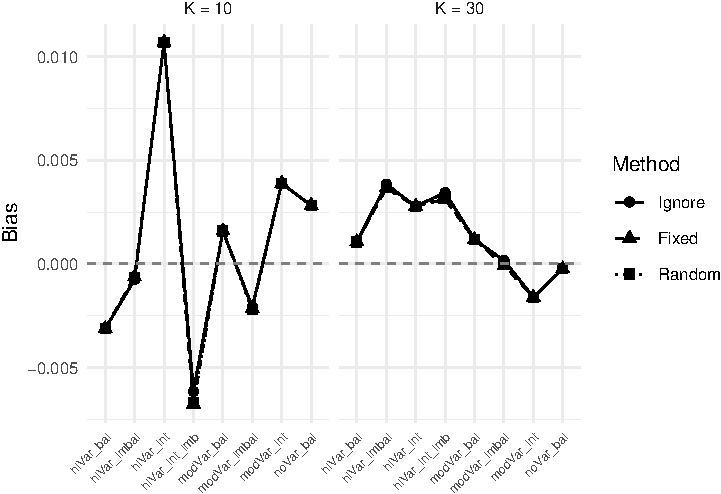
\includegraphics[keepaspectratio,alt={Bias of the treatment effect estimate across scenarios and analytic methods. Dashed line at zero indicates no bias.}]{report_files/report_files/figure-latex/fig-bias-1.pdf}}
\caption{Bias of the treatment effect estimate across scenarios and
analytic methods. Dashed line at zero indicates no bias.}
\end{figure}

\subsection{Power and coverage}\label{power-and-coverage}

\begin{figure}
\centering
\pandocbounded{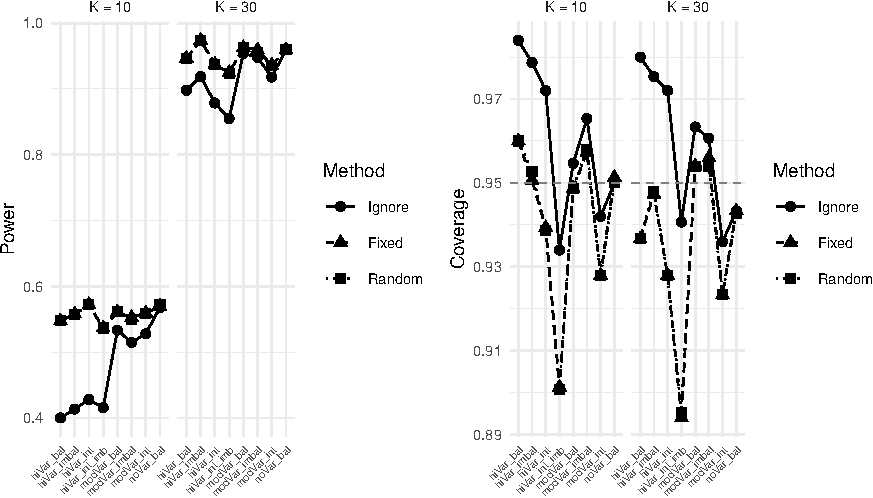
\includegraphics[keepaspectratio,alt={Power (left) and coverage probability (right) across scenarios. Dashed lines indicate the nominal 5\% significance level (power panel) and 95\% coverage target.}]{report_files/report_files/figure-latex/fig-power-1.pdf}}
\caption{Power (left) and coverage probability (right) across scenarios.
Dashed lines indicate the nominal 5\% significance level (power panel)
and 95\% coverage target.}
\end{figure}

\subsection{Impact of imbalanced site
sizes}\label{impact-of-imbalanced-site-sizes}

\begin{figure}
\centering
\pandocbounded{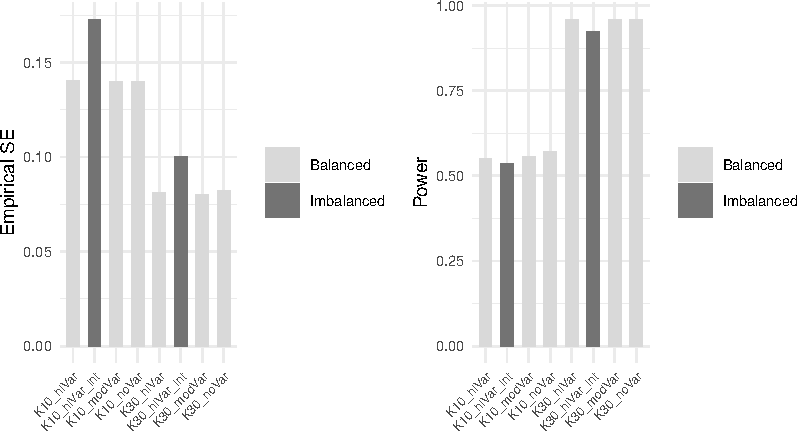
\includegraphics[keepaspectratio,alt={Comparison of balanced versus imbalanced site sizes for the random effects method. Panels show empirical standard error (left) and power (right).}]{report_files/report_files/figure-latex/fig-imbalance-1.pdf}}
\caption{Comparison of balanced versus imbalanced site sizes for the
random effects method. Panels show empirical standard error (left) and
power (right).}
\end{figure}

\section{Discussion}\label{discussion}

The simulation results can be organized around the four research
questions motivating this study.

\textbf{Modeling site effects.} Consistent
with\textsuperscript{\citeproc{ref-chu2011comparing}{7}}
and\textsuperscript{\citeproc{ref-kahanmorris2013continuous}{8}}, the
random effects model attained nominal or near-nominal coverage and the
highest power across nearly all scenarios. The fixed effects model
performed comparably when the number of sites was small (\(K = 10\)) but
lost efficiency with \(K = 30\) due to the large number of nuisance
parameters. Ignoring site effects produced unbiased point estimates but
inflated standard errors when site-level variance was present, leading
to conservative inference and reduced power. These findings support the
random effects model as a robust default for multicenter RCTs, as
recommended
by\textsuperscript{\citeproc{ref-sennlewis2019treatment}{13}}
and\textsuperscript{\citeproc{ref-iche9}{1}}.

\textbf{Failure to adjust for stratification.} The `ignore site' method
effectively represents a failure to adjust for the stratification
variable (site) used in randomization. The overcoverage and power loss
observed under this method confirm the findings
of\textsuperscript{\citeproc{ref-kahanImproperAnalysisTrials2012a}{10}}:
when randomization is stratified by center, the analysis must account
for center to obtain valid inference. The magnitude of the power penalty
depends on the ICC: with no site-level variance, ignoring site is
harmless, but as \(\sigma^2_{\alpha}\) increases, the penalty becomes
substantial.

\textbf{Treatment-by-site interaction.} Introducing random
treatment-by-site interaction (\(\sigma^2_{\gamma} = 0.04\)) increased
the variability of treatment effect estimates across replications for
all methods. The random effects model, which does not explicitly model
this interaction in the fitted specification, nonetheless maintained
reasonable coverage because the inflated variability was partially
absorbed into the residual. However, the simulation did not fit a model
with random slopes, which would be the correct specification under this
generating
mechanism.\textsuperscript{\citeproc{ref-jones1998comparison}{4}}
and\textsuperscript{\citeproc{ref-fedorov2005misleading}{12}} have
argued that some degree of treatment-by-center interaction is
ubiquitous, and that the power to detect it is typically inadequate.
Researchers should plan for its presence rather than test for its
absence.

\textbf{Imbalanced site sizes.} The comparison of balanced versus
imbalanced site sizes reveals that for the random effects model,
moderate imbalance (CV \(\approx 1.1\)) produces only a modest increase
in empirical standard error and a correspondingly small decrease in
power. This finding is consistent
with\textsuperscript{\citeproc{ref-ruvuna2004unequal}{15}}
and\textsuperscript{\citeproc{ref-vierron2009design}{16}}, who showed
that the efficiency loss from unequal site sizes is generally small
unless the imbalance is extreme. The more concerning scenario is when
site size is confounded with site characteristics -- a possibility not
simulated here but discussed
by\textsuperscript{\citeproc{ref-fedorov2005misleading}{12}}
and\textsuperscript{\citeproc{ref-neuhaus2006separating}{14}}. Under
informative site sizes, where larger sites systematically differ from
smaller sites, all methods may produce biased estimates of the
population-average treatment effect.

\textbf{Limitations.} This simulation is restricted to continuous
outcomes analyzed with normal-theory models. Binary and time-to-event
outcomes raise additional complications, including separation in fixed
effects logistic regression with many small
sites\textsuperscript{\citeproc{ref-pickering2007analysis}{5},\citeproc{ref-agresti2000strategies}{17},\citeproc{ref-kahanAccountingCentreeffectsMulticentre2014}{19}}.
The simulation does not incorporate dropout, non-compliance, or
informative site sizes. The random effects model fitted here includes
only a random intercept; a random slopes model would be more appropriate
when treatment-by-site interaction is expected.

\section{Future research}\label{future-research}

Several directions warrant further investigation:

\begin{enumerate}
\def\labelenumi{\arabic{enumi}.}
\item
  \textbf{Random slopes models.} Extending the simulation to include a
  random treatment slope (\(\delta + \gamma_i\) with \(\gamma_i\)
  estimated) would clarify when and how much the random slopes model
  outperforms the random intercept model under genuine treatment
  heterogeneity.
\item
  \textbf{Non-normal outcomes.} Binary and count outcomes require
  generalized linear mixed models or GEE, and the relative performance
  of methods may differ from the continuous case, particularly with
  sparse data per
  site\textsuperscript{\citeproc{ref-agresti2000strategies}{17},\citeproc{ref-kahanAccountingCentreeffectsMulticentre2014}{19}}.
\item
  \textbf{Informative site sizes.} If site size is associated with
  site-level treatment effect (e.g., expert centers enroll more patients
  and also deliver more effective treatment), standard methods may yield
  biased population-average estimates. Inverse-probability weighting by
  site or joint modeling of enrollment and outcome merit
  investigation\textsuperscript{\citeproc{ref-neuhaus2006separating}{14}}.
\item
  \textbf{Small-sample corrections.} With few sites, the Wald-type
  inference from \texttt{lmer} may be anticonservative. Kenward-Roger or
  Satterthwaite denominator degrees of freedom corrections (available in
  \texttt{lmerTest}) should be evaluated across the same scenario grid.
\item
  \textbf{Bayesian approaches.} Hierarchical Bayesian models offer
  partial pooling of site-specific treatment effects, which may
  outperform frequentist random effects models when the number of sites
  is very small\textsuperscript{\citeproc{ref-jones1998comparison}{4}}.
\item
  \textbf{Sample size planning.} Tools that incorporate the design
  effect from multicenter structure, including anticipated ICC and site
  size imbalance, into prospective sample size calculations would
  improve trial
  planning\textsuperscript{\citeproc{ref-vierron2009design}{16},\citeproc{ref-sverdlovSelectingRandomizationMethod2024}{20}}.
\end{enumerate}

\section{References}\label{references}

\subsection{Morris et al.~(2019) ADEMP
Compliance}\label{morris-et-al.-2019-ademp-compliance}

This simulation study was audited against the reporting standards
proposed by Morris, White, and
Crowther\textsuperscript{\citeproc{ref-morris2019using}{18}}. The full
audit is at \texttt{docs/morris-audit-2026-04-17.md}.

\textbf{Verdict:} Partially compliant.

\textbf{Key gaps identified:}

\begin{itemize}
\tightlist
\item
  No Monte Carlo SE on any performance estimate in
  \texttt{summarize\_simulation()}.
\item
  \texttt{R\ =\ 1500} fixed without MCSE-based derivation.
\item
  \texttt{filter(!is.na(est))} silently drops non-converged
  replications, breaking paired comparisons.
\end{itemize}

A remediation plan is documented in the audit file and will be executed
in a subsequent revision.

\vfill

\begin{center}\rule{0.5\linewidth}{0.5pt}\end{center}

\emph{Rendered on 2026-05-11 at 18:42 PDT.}\\
\emph{Source:
\texttt{\textasciitilde{}/prj/res/07-multicenter-rct/multicenterrct/analysis/report/report.Rmd}}

\protect\phantomsection\label{refs}
\begin{CSLReferences}{0}{1}
\bibitem[\citeproctext]{ref-iche9}
\CSLLeftMargin{1. }%
\CSLRightInline{International Council for Harmonisation. ICH {E9}:
Statistical principles for clinical trials. Published online 1998.
\url{https://database.ich.org/sites/default/files/E9_Guideline.pdf}}

\bibitem[\citeproctext]{ref-localio2001adjustments}
\CSLLeftMargin{2. }%
\CSLRightInline{Localio AR, Berlin JA, Ten Have TR, Kimmel SE.
Adjustments for center in multicenter studies: An overview. \emph{Annals
of Internal Medicine}. 2001;135(2):112-123.
doi:\href{https://doi.org/10.7326/0003-4819-135-2-200107170-00012}{10.7326/0003-4819-135-2-200107170-00012}}

\bibitem[\citeproctext]{ref-senn1998controversies}
\CSLLeftMargin{3. }%
\CSLRightInline{Senn SJ. Some controversies in planning and analysing
multi-centre trials. \emph{Statistics in Medicine}.
1998;17(15-16):1753-1765.
doi:\href{https://doi.org/10.1002/(SICI)1097-0258(19980815/30)17:15/16\%3C1753::AID-SIM977\%3E3.0.CO;2-X}{10.1002/(SICI)1097-0258(19980815/30)17:15/16\textless1753::AID-SIM977\textgreater3.0.CO;2-X}}

\bibitem[\citeproctext]{ref-jones1998comparison}
\CSLLeftMargin{4. }%
\CSLRightInline{Jones B, Teather D, Wang J, Lewis JA. A comparison of
various estimators of a treatment difference for a multi-centre clinical
trial. \emph{Statistics in Medicine}. 1998;17(15-16):1767-1777.
doi:\href{https://doi.org/10.1002/(SICI)1097-0258(19980815/30)17:15/16\%3C1767::AID-SIM978\%3E3.0.CO;2-H}{10.1002/(SICI)1097-0258(19980815/30)17:15/16\textless1767::AID-SIM978\textgreater3.0.CO;2-H}}

\bibitem[\citeproctext]{ref-pickering2007analysis}
\CSLLeftMargin{5. }%
\CSLRightInline{Pickering RM, Weatherall M. The analysis of continuous
outcomes in multi-centre trials with small centre sizes.
\emph{Statistics in Medicine}. 2007;26(30):5445-5456.
doi:\href{https://doi.org/10.1002/sim.3068}{10.1002/sim.3068}}

\bibitem[\citeproctext]{ref-bates2015lme4}
\CSLLeftMargin{6. }%
\CSLRightInline{Bates D, Mächler M, Bolker B, Walker S. Fitting linear
mixed-effects models using \texttt{lme4}. \emph{Journal of Statistical
Software}. 2015;67(1):1-48.
doi:\href{https://doi.org/10.18637/jss.v067.i01}{10.18637/jss.v067.i01}}

\bibitem[\citeproctext]{ref-chu2011comparing}
\CSLLeftMargin{7. }%
\CSLRightInline{Chu R, Thabane L, Ma J, Holbrook A, Pullenayegum E,
Devereaux PJ. Comparing methods to estimate treatment effects on a
continuous outcome in multicentre randomized controlled trials: A
simulation study. \emph{BMC Medical Research Methodology}. 2011;11:21.
doi:\href{https://doi.org/10.1186/1471-2288-11-21}{10.1186/1471-2288-11-21}}

\bibitem[\citeproctext]{ref-kahanmorris2013continuous}
\CSLLeftMargin{8. }%
\CSLRightInline{Kahan BC, Morris TP. Analysis of multicentre trials with
continuous outcomes: When and how should we account for centre effects?
\emph{Statistics in Medicine}. 2013;32(7):1136-1149.
doi:\href{https://doi.org/10.1002/sim.5667}{10.1002/sim.5667}}

\bibitem[\citeproctext]{ref-islam2024accounting}
\CSLLeftMargin{9. }%
\CSLRightInline{Islam S, Bangdiwala SI. Accounting for center-level
effects in multicenter randomized controlled trials. \emph{Trials}.
2024;25:390.
doi:\href{https://doi.org/10.1186/s13063-024-08202-w}{10.1186/s13063-024-08202-w}}

\bibitem[\citeproctext]{ref-kahanImproperAnalysisTrials2012a}
\CSLLeftMargin{10. }%
\CSLRightInline{Kahan BC, Morris TP. Improper analysis of trials
randomised using stratified blocks or minimisation. \emph{Statistics in
Medicine}. 2012;31(4):328-340.
doi:\href{https://doi.org/10.1002/sim.4431}{10.1002/sim.4431}}

\bibitem[\citeproctext]{ref-kahanAdjustingMultiplePrognostic2013}
\CSLLeftMargin{11. }%
\CSLRightInline{Kahan BC, Morris TP. Adjusting for multiple prognostic
factors in the analysis of randomised trials. \emph{BMC Medical Research
Methodology}. 2013;13(1):99.
doi:\href{https://doi.org/10.1186/1471-2288-13-99}{10.1186/1471-2288-13-99}}

\bibitem[\citeproctext]{ref-fedorov2005misleading}
\CSLLeftMargin{12. }%
\CSLRightInline{Fedorov V, Jones B. Are certain multicenter randomized
clinical trial structures misleading clinical and policy decisions?
\emph{Contemporary Clinical Trials}. 2005;26(5):518-529.
doi:\href{https://doi.org/10.1016/j.cct.2005.05.002}{10.1016/j.cct.2005.05.002}}

\bibitem[\citeproctext]{ref-sennlewis2019treatment}
\CSLLeftMargin{13. }%
\CSLRightInline{Senn SJ, Lewis RJ. Treatment effects in multicenter
randomized clinical trials. \emph{JAMA}. 2019;321(12):1211-1212.
doi:\href{https://doi.org/10.1001/jama.2019.1553}{10.1001/jama.2019.1553}}

\bibitem[\citeproctext]{ref-neuhaus2006separating}
\CSLLeftMargin{14. }%
\CSLRightInline{Neuhaus JM, McCulloch CE. Separating between- and
within-cluster covariate effects by using conditional and partitioning
methods. \emph{Journal of the Royal Statistical Society: Series B}.
2006;68(5):859-872.
doi:\href{https://doi.org/10.1111/j.1467-9868.2006.00570.x}{10.1111/j.1467-9868.2006.00570.x}}

\bibitem[\citeproctext]{ref-ruvuna2004unequal}
\CSLLeftMargin{15. }%
\CSLRightInline{Ruvuna F. Unequal center sizes, sample size, and power
in multicenter clinical trials. \emph{Drug Information Journal}.
2004;38(4):387-394.
doi:\href{https://doi.org/10.1177/009286150403800409}{10.1177/009286150403800409}}

\bibitem[\citeproctext]{ref-vierron2009design}
\CSLLeftMargin{16. }%
\CSLRightInline{Vierron E, Giraudeau B. Design effect in multicenter
studies: Gain or loss of power? \emph{BMC Medical Research Methodology}.
2009;9:39.
doi:\href{https://doi.org/10.1186/1471-2288-9-39}{10.1186/1471-2288-9-39}}

\bibitem[\citeproctext]{ref-agresti2000strategies}
\CSLLeftMargin{17. }%
\CSLRightInline{Agresti A, Hartzel J. Strategies for comparing
treatments on a binary response with multi-centre data. \emph{Statistics
in Medicine}. 2000;19(8):1115-1139.
doi:\href{https://doi.org/10.1002/(SICI)1097-0258(20000430)19:8\%3C1115::AID-SIM408\%3E3.0.CO;2-X}{10.1002/(SICI)1097-0258(20000430)19:8\textless1115::AID-SIM408\textgreater3.0.CO;2-X}}

\bibitem[\citeproctext]{ref-morris2019using}
\CSLLeftMargin{18. }%
\CSLRightInline{Morris TP, White IR, Crowther MJ. Using simulation
studies to evaluate statistical methods. \emph{Statistics in Medicine}.
2019;38(11):2074-2102.
doi:\href{https://doi.org/10.1002/sim.8086}{10.1002/sim.8086}}

\bibitem[\citeproctext]{ref-kahanAccountingCentreeffectsMulticentre2014}
\CSLLeftMargin{19. }%
\CSLRightInline{Kahan BC. Accounting for centre-effects in multicentre
trials with a binary outcome -- when, why, and how? \emph{BMC Medical
Research Methodology}. 2014;14(1):20.
doi:\href{https://doi.org/10.1186/1471-2288-14-20}{10.1186/1471-2288-14-20}}

\bibitem[\citeproctext]{ref-sverdlovSelectingRandomizationMethod2024}
\CSLLeftMargin{20. }%
\CSLRightInline{Sverdlov O, Ryeznik Y, Anisimov V, et al. Selecting a
randomization method for a multi-center clinical trial with stochastic
recruitment considerations. \emph{BMC Medical Research Methodology}.
2024;24(1):52.
doi:\href{https://doi.org/10.1186/s12874-023-02131-z}{10.1186/s12874-023-02131-z}}

\end{CSLReferences}

\end{document}
